\section{Registrar Unidad Temática}

Para registrar una Unidad Temática  correspondiente a una Unidad de Aprendizaje, primero se da click en en la pestaña \IUbutton{Ver Tareas}. y posteriormente en el botón \IUbutton{Unidad Temática} y la siguiente pantalla será desplegada:

\hypertarget{RUT}{\begin{figure}[!h]
    \centering
    \hypertarget{9}{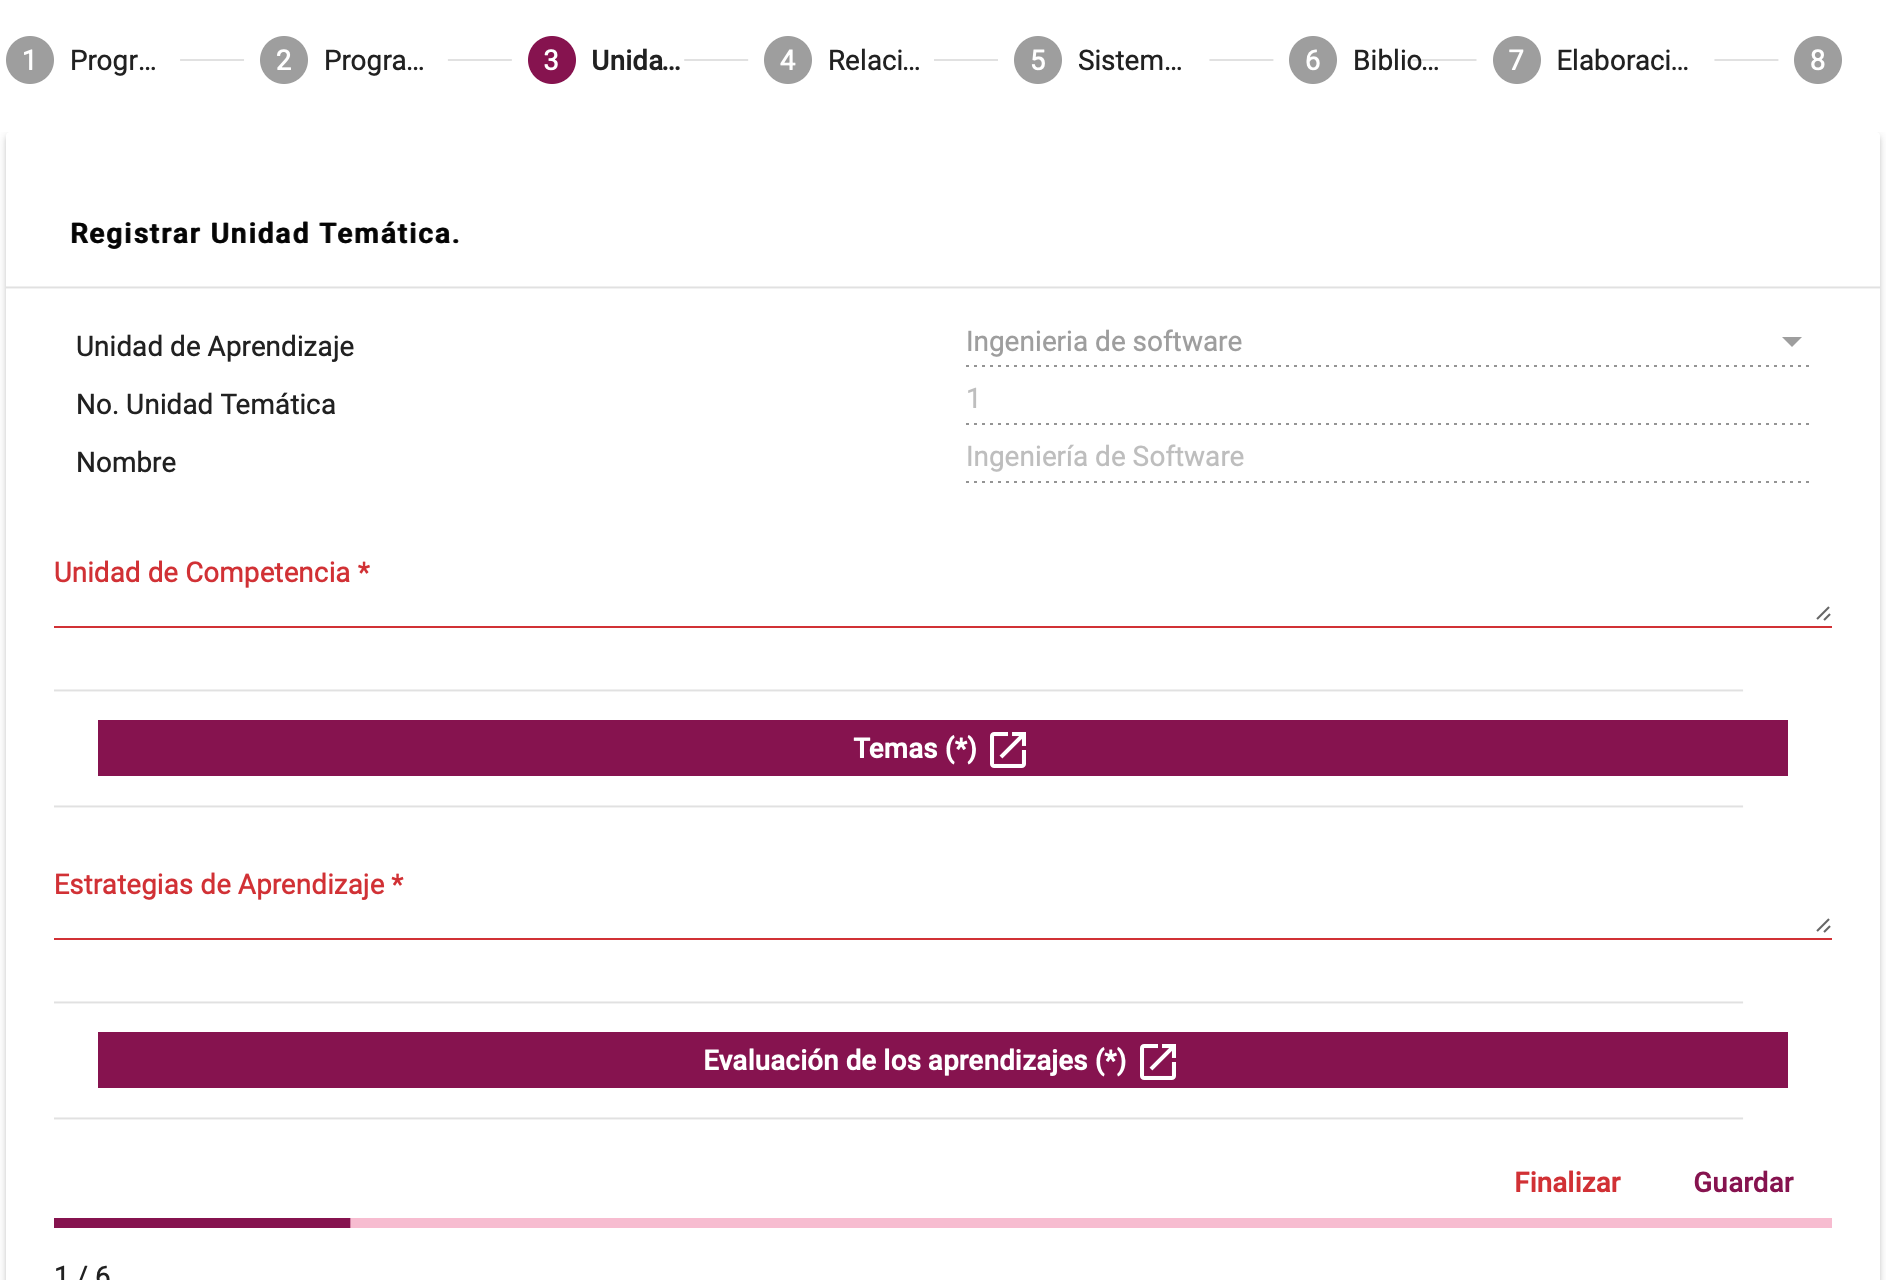
\includegraphics[width=0.5\linewidth]{images/SP6/RegistrarUT.png}}
    \caption{Pantalla para Registrar Unidad Temática}
\end{figure}
}


Los campos desplegados en el formulario deberan ser llenados por el Docente.

Si el Docente desea:

\begin{itemize}
    \item Registrar Temas. El Docente debe dar click sobre el botón \IUbutton{Temas(*)}. Posteriormente consulte \hyperlink{RegistrarTema}{Registrar Tema}
    \item Registrar Evaluación de los Aprendizajes. El Docente debe dar click sobre el botón \IUbutton{Evaluación de los Aprendizajes (*)}. Posteriormente consulte \hyperlink{RegistrarEvalAprend}{Registrar Evaluación y Acreditación}
    \item Registrar las siguientes Unidades Temáticas. Dar click al botón:
    \begin{figure}[!hbtp]
    \centering
    
\includegraphics[width=0.05\linewidth]{images/SP6/Flecha.png}
    \caption{Flecha para Continuar.} 
    
    De esta manera se despliegan nuevos campos para una nueva Unidad Temática. 
\end{figure}
    
\end{itemize}

Al llenar todos los datos correctamente, el Docente da click en el botón:

Para concluir el registro. Revisar \hyperlink{GuardarFinalizar}{Guardar y/o Finalizar}
Si hay errores checar \hyperlink{Errores}{Posibles Errores}


\pagebreak

\hypertarget{RegistrarTema}{\subsection{Registrar Tema}}
Para registrar un Tema correspondiente a una Unidad Temática, se debe acceder por medio del botón \IUbutton{Temas} de la pantalla \hyperlink{RUT}{Registrar Unidad Temática}. Posteriormente se muestra la siguiente pantalla:

\hypertarget{RTema}{}
\begin{figure}[!hbtp]
    \centering
    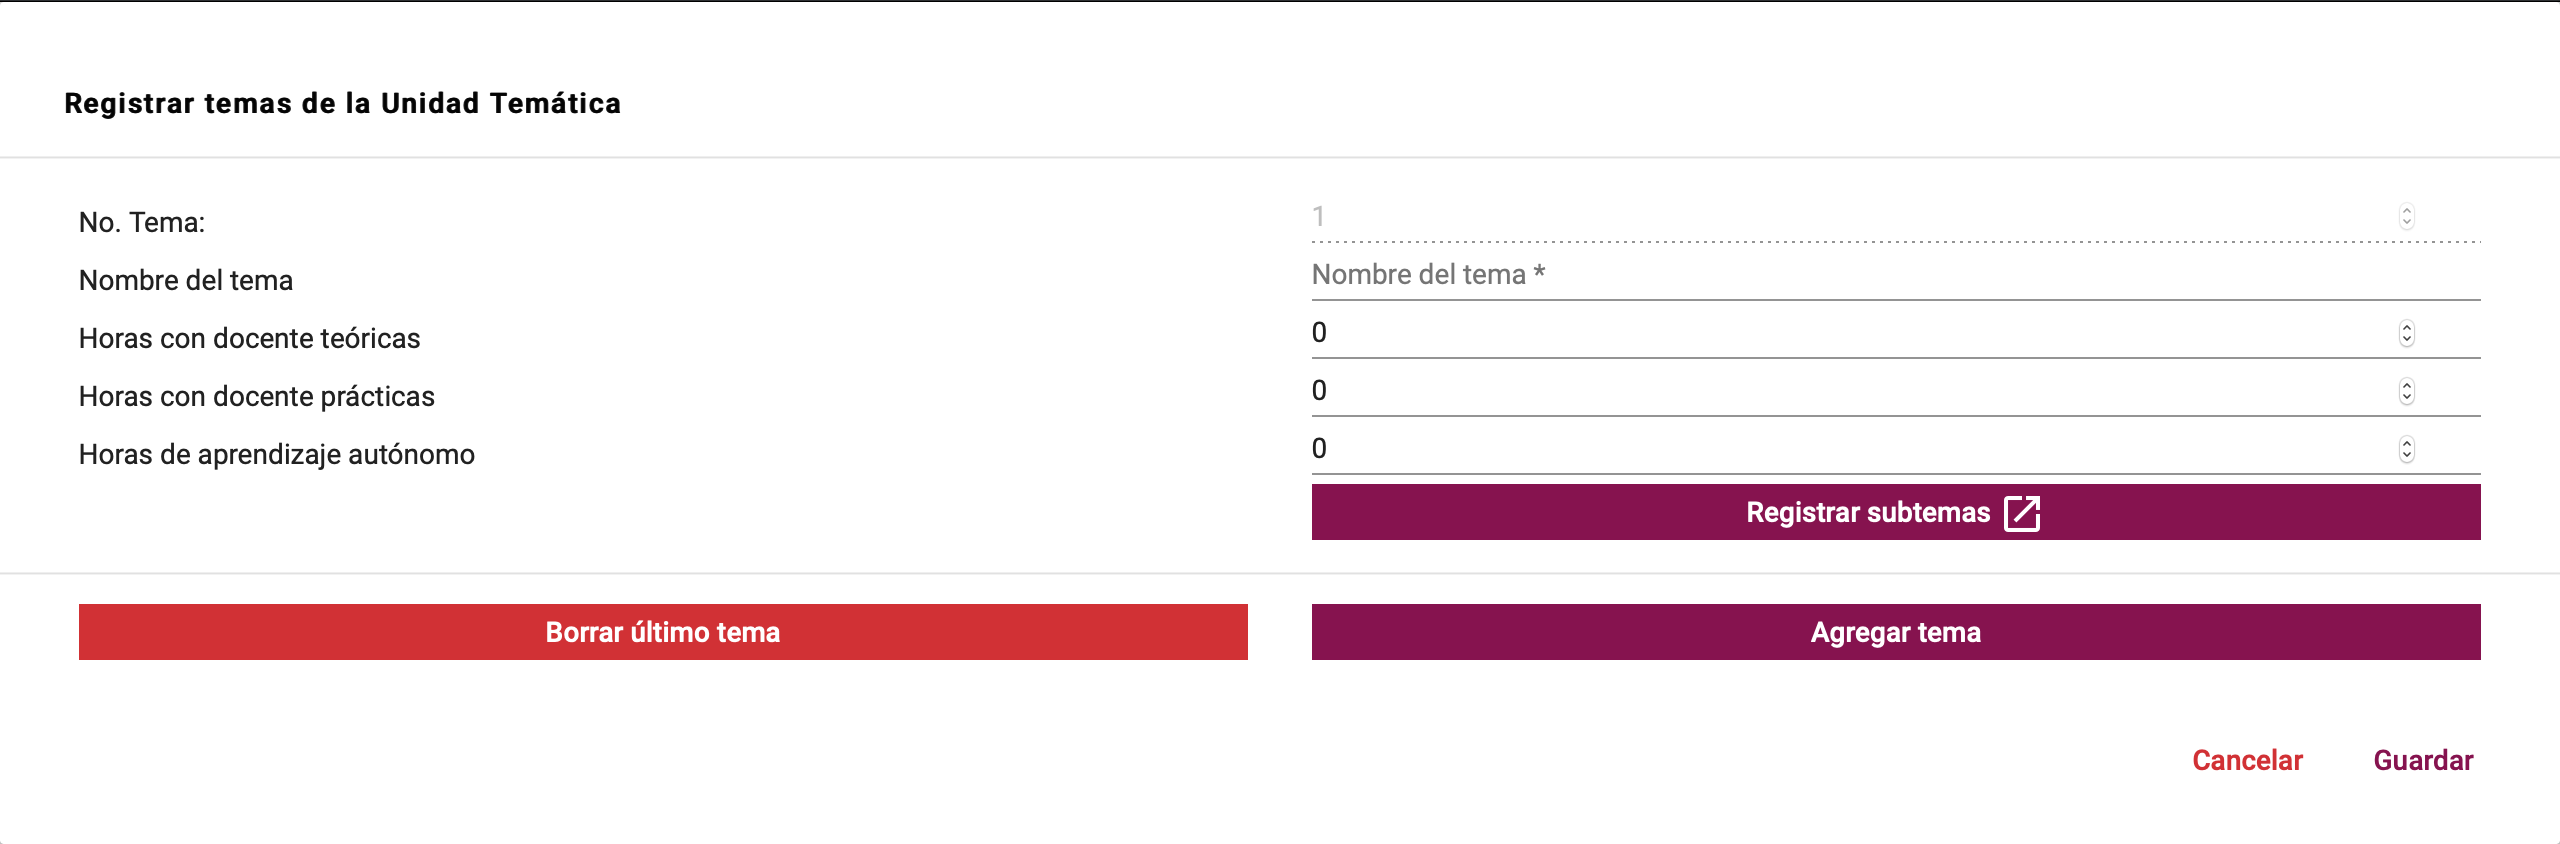
\includegraphics[width=0.7\linewidth]{images/SP6/RegistrarTema.png}
    \caption{Pantalla para Registrar Temas.} 
\end{figure}

Los campos desplegados en el formulario deben ser llenados por el Docente.

Si el docente desea:
\begin{itemize}
    \item Registrar Subtema. Checar \hyperlink{RegistrarSubtema}{Registrar Subtema}.
    \item Agregar Tema. El docente da click al botón:
    \begin{figure}[!hbtp]
    \centering
    
\includegraphics[width=0.4\linewidth]{images/SP6/AgregarTema.png}
    \caption{Pantalla para Agregar Temas.} 
    \end{figure}
    Se agregará nuevos campos para un tema. Posteriormente el docente llena los nuevos campos.
    \item Eliminar Último Tema. El docente da click: al botón:
    \begin{figure}[!hbtp]
    \centering
    
\includegraphics[width=0.4\linewidth]{images/SP6/EliminarTema.png}
    \caption{Pantalla para Eliminar Temas.} 
    \end{figure}
    Se eliminará el último tema. Esto no aplica si solo hay un tema.
\end{itemize}

Para concluir el registro. Revisar \hyperlink{AceptarCancelar}{Aceptar o Cancelar}
Si hay errores checar \hyperlink{Errores}{Posibles Errores}

\pagebreak
\hypertarget{RegistrarSubtema}{\subsection{Registrar Subtema}}



Para registrar un Subtema correspondiente a Tema, se debe acceder por medio del botón \IUbutton{Subtema} de la pantalla \hyperlink{RTema}{Registrar Tema}. Posteriormente se muestra la siguiente pantalla:

\begin{figure}[!hbtp]
    \centering
    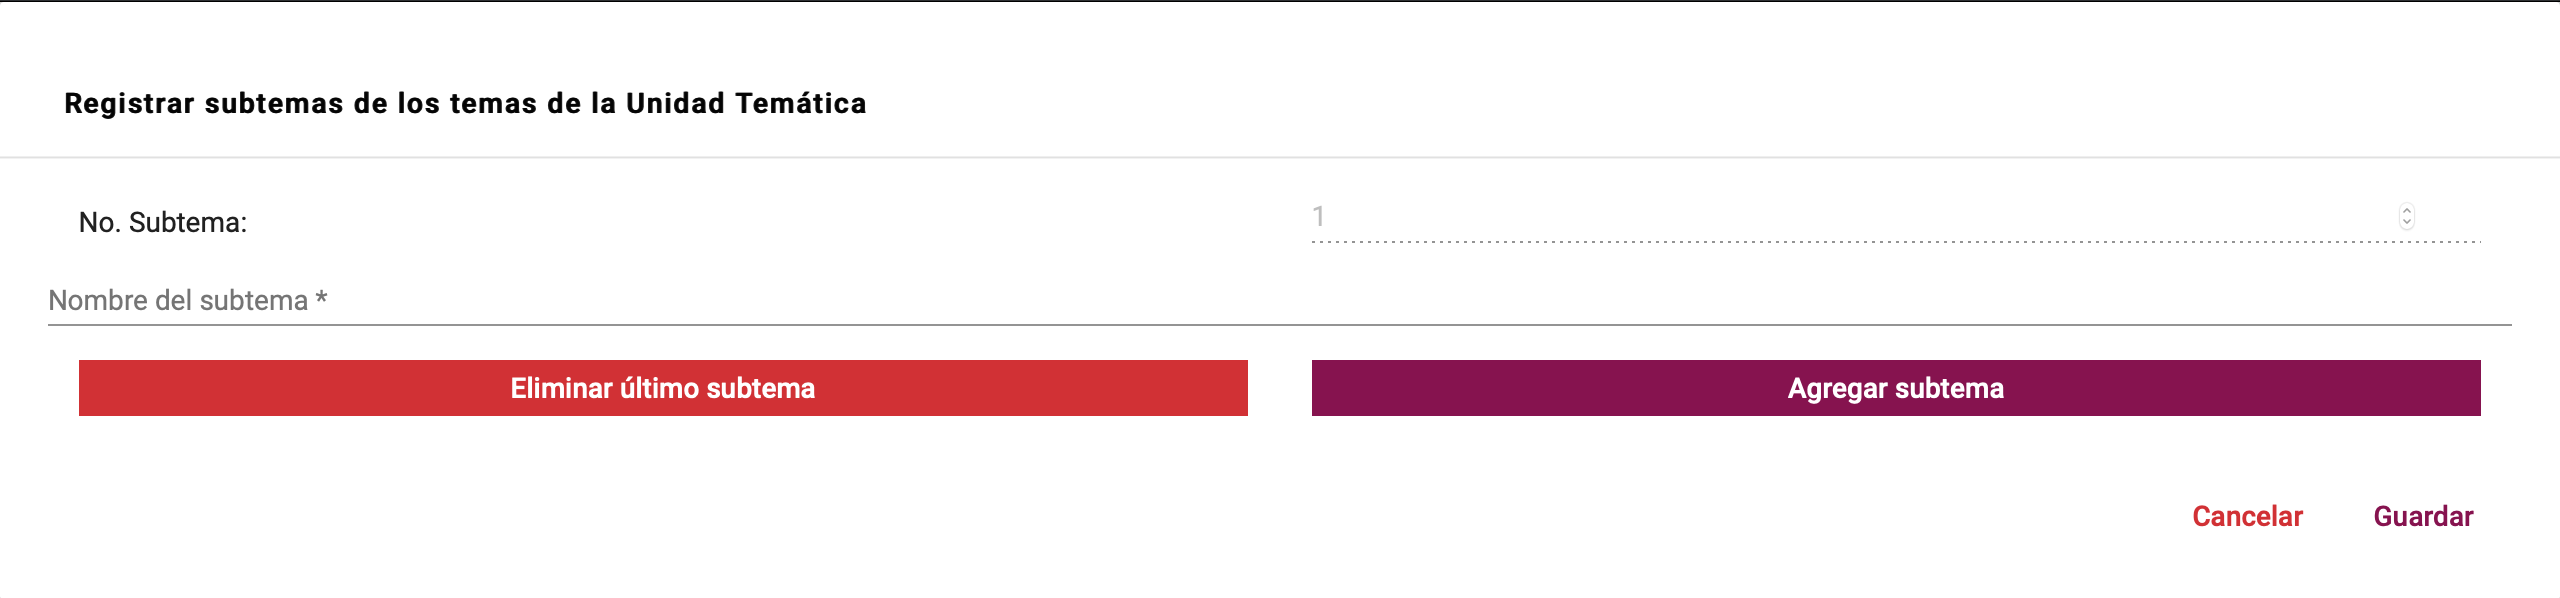
\includegraphics[width=0.7\linewidth]{images/SP6/RegistrarSubtema.png}
    \caption{Pantalla para Registrar Subtemas.} 
\end{figure}

Los campos desplegados en el formulario deben ser llenados por el Docente.

Si el docente desea:
\begin{itemize}
    \item Agregar Subtema. El docente da click al botón:
    \begin{figure}[!hbtp]
    \centering
    
\includegraphics[width=0.4\linewidth]{images/SP6/AgregarSubtema.png}
    \caption{Pantalla para Agregar Subtemas.} 
    \end{figure}
    Se agregan nuevos campos para un tema. Posteriormente el docente llena los nuevos campos.
    \item Eliminar Último Subtema. El docente da click: al botón:
    \begin{figure}[!hbtp]
    \centering
    
\includegraphics[width=0.4\linewidth]{images/SP6/EliminarSubtema.png}
    \caption{Pantalla para Eliminar Temas.} 
    \end{figure}
    Se elimina el último subtema. Esto no aplica si solo hay un subtema.
\end{itemize}

Para concluir el registro. Revisar \hyperlink{AceptarCancelar}{Aceptar o Cancelar}
Si hay errores checar \hyperlink{Errores}{Posibles Errores}

\pagebreak
\hypertarget{RegistrarEvalAprend}{\subsection{Registrar Evaluación de los Aprendizajes}}

Para registrar la Evaluación de los Aprendizajes correspondiente a una Unidad Temática, se debe acceder por medio del botón \IUbutton{Evaluación de los Aprendizajes} de la pantalla \hyperlink{RUT}{Registrar Unidad Temática}. Posteriormente se muestra la siguiente pantalla:

\hypertarget{REvalApre}{}
\begin{figure}[!hbtp]
    \centering
    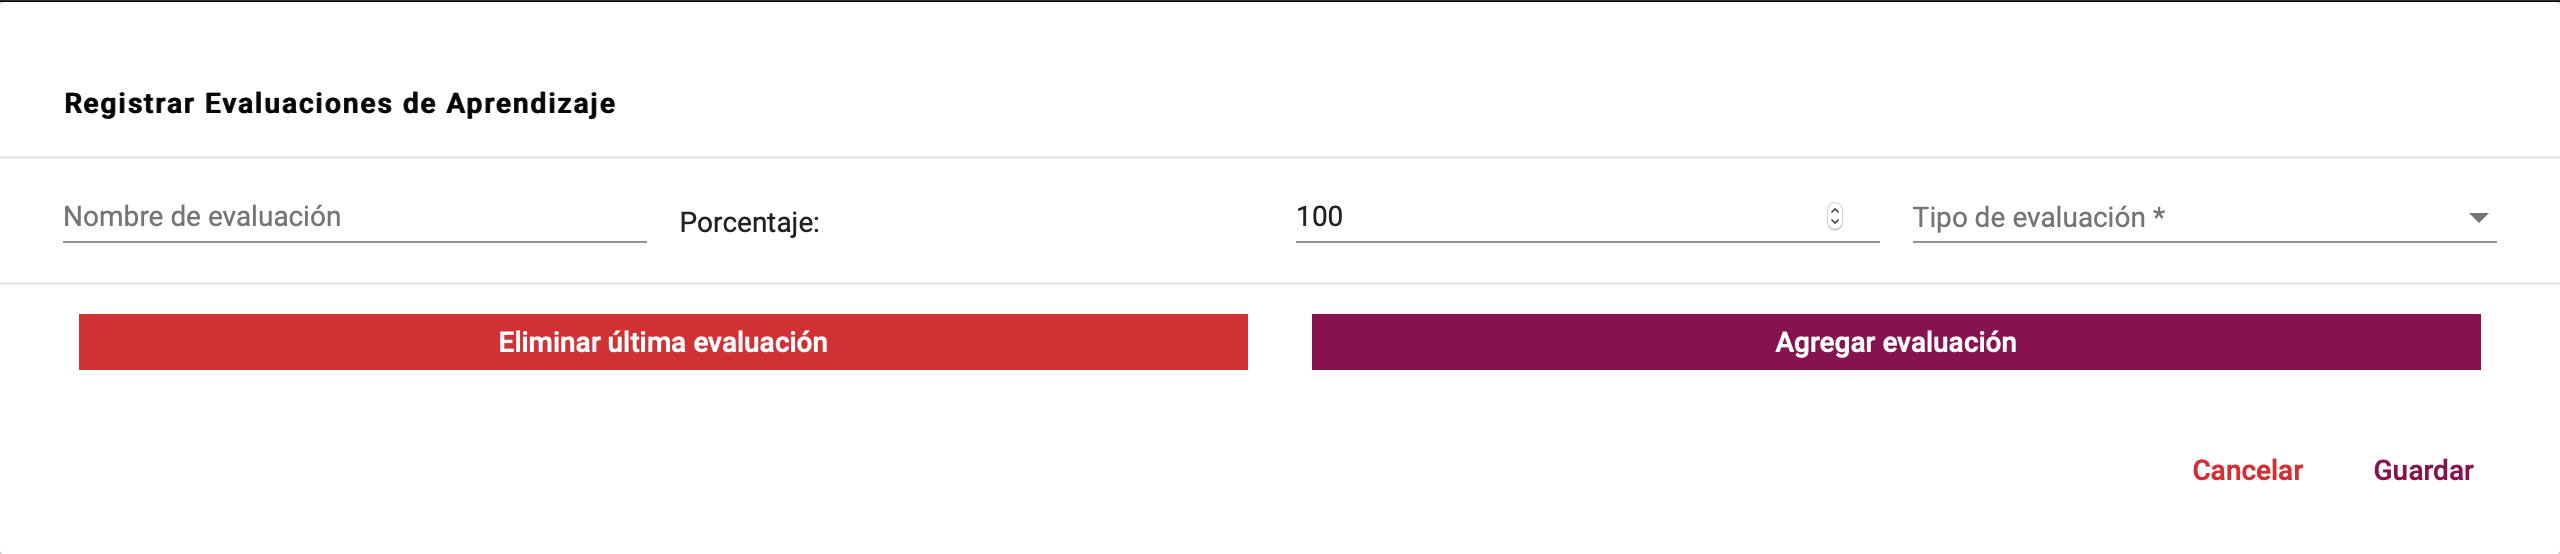
\includegraphics[width=0.7\linewidth]{images/SP6/RegistrarEvadeApren.png}
    \caption{Pantalla para Registrar Temas.} 
\end{figure}

Los campos desplegados en el formulario deben ser llenados por el Docente.

Si el docente desea:
\begin{itemize}
    \item Agregar Evaluación. El docente da click al botón:
    \begin{figure}[!hbtp]
    \centering
    
\includegraphics[width=0.4\linewidth]{images/SP6/AgregarEval.png}
    \caption{Pantalla para Agregar Evaluación.} 
    \end{figure}
    Se agregan nuevos campos para una Evaluación. Posteriormente el docente llena los nuevos campos.
    \item Eliminar Última Evaluación. El docente da click: al botón:
    \begin{figure}[!hbtp]
    \centering
    
\includegraphics[width=0.4\linewidth]{images/SP6/ElimarEval.png}
    \caption{Pantalla para Eliminar Evaluación.} 
    \end{figure}
    Se eliminará el último Evaluación. Esto no aplica si solo hay una Evaluación.
\end{itemize}

Para concluir el registro. Revisar \hyperlink{GuardarFinalizar}{Guardar y Finalizar}
Si hay errores checar \hyperlink{Errores}{Posibles Errores}
\pagebreak

